\section{Leaf application details}\label{sec:application-details}

\subsection{Data and computation}

The sequence selected in \cref{sec:application} has sample identifier
$1818$. Of its $16$ raw records, two are manually flagged and removed
by the source study's quality filters. The third excluded record is
the dark measurement, for which insufficient dark adaptation prevents
estimation of dark respiration \citep{rogers2019arctic}.

The marginal-likelihood optimization uses rank $32$ and padding
$L=2$, with the resulting estimates carried into the rank-$24$
model in \cref{eq:application-model}. The constrained fit uses four Stan chains,
each with $1{,}500$ warm-up and $3{,}000$ retained iterations, a dense
metric, target acceptance $0.99$, maximum tree depth $12$, and threshold
tolerance $10^{-8}$. The unconstrained fit uses $20{,}000$ independent
Gaussian posterior draws.

\paragraph{MCMC diagnostics.}
We assess mixing across all $80$ scalar outputs of the constrained fit,
including the coefficient coordinates, reconstructed coefficients,
log density, and quantities used in threshold evaluation and
reconstruction. Across these outputs, the maximum rank-normalized
split $\widehat R$ is $1.0007$, and the minimum bulk and tail effective
sample sizes are $5{,}616$ and $7{,}866$, respectively. None of the
$12{,}000$ retained iterations has a divergence or reaches the
tree-depth limit, and the minimum energy Bayesian fraction of missing
information (E-BFMI) across chains is $0.9642$. These diagnostics
reveal no warning about mixing in the monitored quantities. The
predictive checks below separately assess agreement with the
observation model.

\subsection{Curvature inference}

To complement the marginal-gain comparison in
\cref{fig:light-response}, \cref{fig:curvature} shows how rapidly
marginal gain changes with irradiance. Concavity restricts the sign of this second
derivative while allowing its magnitude to vary across the range.
The pointwise intervals describe uncertainty about that local rate
of change.
\begin{figure}[htbp]
\centering
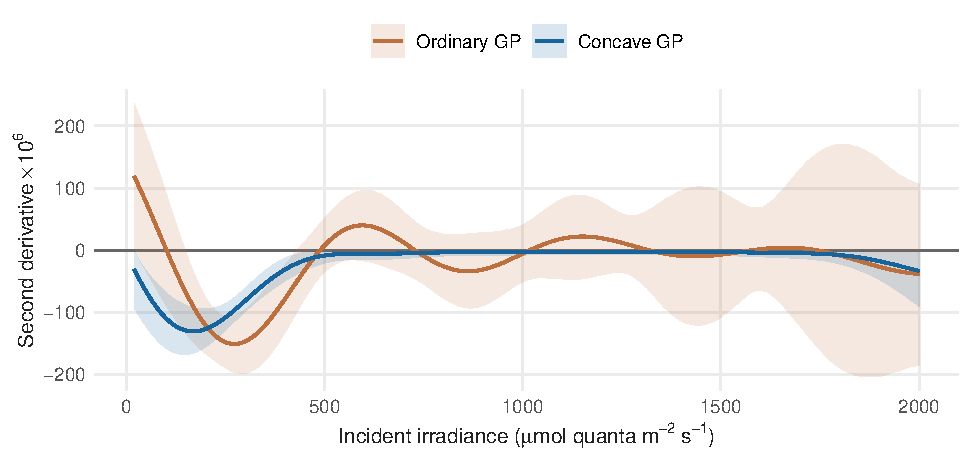
\includegraphics[width=\textwidth]{figures/curvature.pdf}
\caption[Leaf response curvature]{Second derivative of net assimilation
with respect to irradiance for the selected leaf, multiplied by $10^6$,
with unscaled units of assimilation per squared irradiance.
Orange and blue lines show ordinary Gaussian and concavity-conditioned
posterior means and pointwise $95\%$ equal-tail intervals under the same
covariance and noise estimates. The intervals describe latent curvature,
exclude measurement noise, and do not give simultaneous coverage,
while the horizontal reference marks zero.}
\label{fig:curvature}
\end{figure}

\subsection{Predictive checks}

For each posterior curve from either fit, we generate one independent
replicate dataset at the observed irradiances using the Gaussian
observation model in \cref{eq:application-model}. Define
$r_i(A)=(y_i-A(q_i))/\sigma_\varepsilon$ and let $\pi$ order
the measurements by time. The two discrepancies are the maximum
absolute standardized residual and the absolute sum of adjacent
residual products,
\[
 D_{\max}(\boldsymbol y,A)=\max_i|r_i(A)|,\qquad
 D_{\mathrm{seq}}(\boldsymbol y,A)=
 \left|\sum_{i=1}^{n-1}r_{\pi(i)}(A)r_{\pi(i+1)}(A)\right|.
\]
\begin{samepage}
For either discrepancy $D$, we average the indicator of a replicated
value at least as large as the observed value over all curves from
the corresponding fit. This upper-tail fraction estimates
$P(D(\boldsymbol Y^{\mathrm{rep}},A)\geq
D(\boldsymbol y,A)\mid\boldsymbol y)$, with observed and replicated
discrepancies evaluated using the same posterior curve.
\end{samepage}

The upper-tail fractions for $D_{\max}$ are \AppPpcMaximum\ under
concavity and \OrdPpcMaximum\ without the restriction, while
$D_{\mathrm{seq}}$ gives \AppPpcSequence\ and \OrdPpcSequence,
respectively. Neither comparison shows pronounced disagreement,
although $13$ records provide limited information about dependence
or changes in measurement variance.
Because irradiance decreases with time, the sequence discrepancy
cannot distinguish temporal dependence from systematic response error
across irradiance. Both fractions reuse the fitting data and therefore
are not calibrated test probabilities.
